\documentclass[12pt]{report}
 
%%%%%%%%%%%%%%%%%%%%%%%%%%%%%%%%%%%%%%%%%%%%%%%%%%%%%%%%%%%%%%%%%%%%%%%%%%%%%%%%%%%%\usepackage[margin=1in]{geometry} 
\usepackage{amsmath,amsthm,amssymb}
\usepackage[utf8]{inputenc}
\usepackage{amsmath}
\usepackage[shortlabels]{enumitem}
\usepackage{mathtools}
\usepackage{personalcommands}
\usepackage{amsfonts}
\usepackage{float}
\usepackage{epigraph}
\usepackage{lipsum}
\usepackage{parskip}
\usepackage[spanish]{babel}
\usepackage{tikz}
\usetikzlibrary{babel}
\usepackage{csquotes}
\usepackage{xcolor}
\usepackage[framemethod=tikz,xcolor=true]{mdframed}
\usepackage[new]{old-arrows}
%%%%%%%%%%%%%%%%%%%%%%%%%%%%%%%%%%%%%%%%%%%%%%%%%%%%%%%%%%%%%%%%%%%%%%%%%%%%%%%%%%
\begin{document}

Sean las relaciones $R$ y $S$ con los siguientes parámetros:

\begin{center}
\begin{tabular}{|c|c|}
\hline 
R(a,b,c) & S(d,e,b) \\ 
\hline 
N(R)=1000 & N(S)=5000 \\ 
\hline 
Size(a)=20 &   \\ 
\hline 
Size(b)=30 & Size(b)=30 \\ 
\hline 
Size(c)=100 &   \\ 
\hline 
  & Size(d)=20 \\ 
\hline 
  & Size(e)=40 \\ 
\hline 
V(R,a)=1000 &   \\ 
\hline 
V(R,b)=200 & V(S,b)=500 \\ 
\hline 
V(R,c)=20 &   \\ 
\hline 
  & V(S,d)=5000 \\ 
\hline 
  & V(S,e)=40 \\ 
\hline 
\end{tabular} 
\end{center}
donde $a$ es la llave primaria de $R$ y $d$ es la llave primaria de $S$, y donde \textbf{no} existe una relación de llave externa entre las relaciones $R$ y $S$, aunque ambas tengan un atributo común en nombre y dominio (con valores comunes) $b$.

Teniendo en cuenta que el $B=4KB$, $C=40B$, que se usa \textbf{bloqueo fijo}, que los \textbf{bloques} son \textbf{homogéneos}, que en memoria cabe únicamente un bloque de cada relación o resultado de operación intermedia, y considerando que las operaciones de \textbf{proyección y selección 'no respetan' índices} (es decir, si las relaciones sobre las que se aplica la operación tienen un índice, el resultado de la misma no está indexado).

\textbf{Ejercicio 1.} Construye el plan lógico que se generaría para la consulta:
\[
\sigma_{e=e_k}\left(\Pi_{a,e}(R\;JOIN\;S)\right)
\]
El plano lógico resultante sería:
\begin{center}
\begin{tikzpicture}[scale=0.4]
\draw (0,0) node[anchor=north] {$\sigma_{e=e_k}$};
\draw (0,-1.1)-- (0,-3);
\draw (0,-3) node[anchor=north] {$\Pi_{a,e}$};
\draw (0,-4.3)-- (0,-6);
\draw (0,-6) node[anchor=north] {$JOIN$};
\draw (0,-7.2)-- (-3,-9);
\draw (-3,-9) node[anchor=north] {$R$};
\draw (0,-7.2)-- (3,-9);
\draw (3,-9) node[anchor=north] {$S$};
\end{tikzpicture}
\end{center}
% codigo para dibujar funciones tests
%\begin{tikzpicture}[scale=0.5]
%\node[inner sep=0pt] (russell) at (0,0)
%    {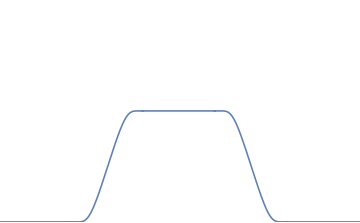
\includegraphics[scale=1]{img/flat.png}};
%\draw (-8,-7.75)-- (8,-7.75);
%\draw[-,dashed] (-5,0)-- (5,0); 
%\draw (-6,0) node[anchor=north] {$1$};
%\draw[-,dashed] (-7,-8.25) -- (-7,-7.25);
%\draw (-7,-8.5) node [anchor=north] {$a$};
%\draw[-,dashed] (0,-8.25) -- (0,-7.25);
%\draw (0,-8.5) node [anchor=north] {$b$};
%\end{tikzpicture}


\end{document}

